\subsection{MetaPredict}

Top scoring pairs (TSP) is a robust algorithm for predicting gene-expression profiles,
which adopts nonparametric rank-based prediction rule.
The MetaPredict is a meta-analysis version of the TSP algorithm that combines multiple transcriptomic studies to build a prediction model and shows improved 
prediction accuracy as compared to single study analysis.
The R package for the MetaPredict module can be found at \url{https://github.com/metaOmics/MetaPredict}.

The homepage for MetaPredict is shown in Figure \ref{fig:MetaPredictmainpage}.
Under advanced options,  there is one drop-down menu (``Methods for MetaPredict") {\color{red} (1)}, 
``Max number of top scoring pairs (K)" {\color{red} (2)}, 
``Number of cores for parallel computing" {\color{red} (3)}.
These will be introduced shortly, 
but the users are not advised to change them unless they know about the algorithm.
The necessary parameters include ``Number of top scoring pairs (K)" {\color{red} (7)}), 
three character entries (``Please select TWO labels to cluster" {\color{red} (4)}, 
``Please select studies for training" {\color{red} (5)}, 
and ``Please select studies for testing") {\color{red} (6)}, 
and two executing tabs (``Train model" and ``Predict"). 

\subsubsection{Procedure}

\begin{figure}[H]
\begin{center}
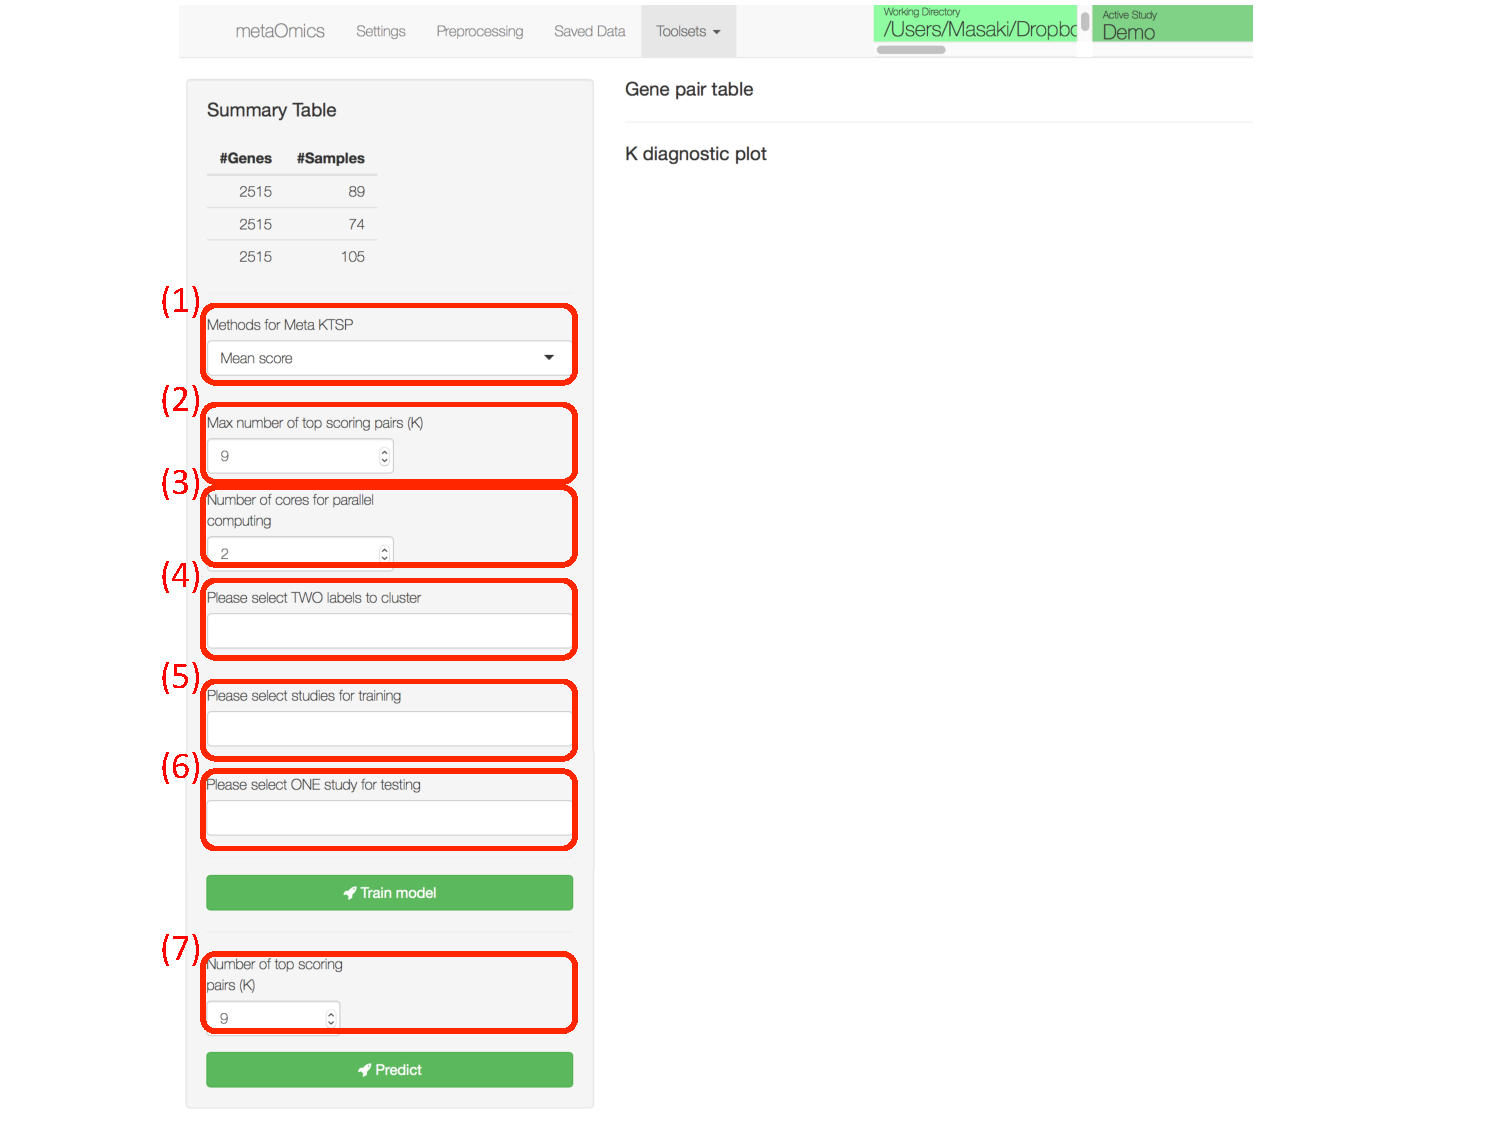
\includegraphics[scale=0.5]{./figure/MetaPredict/MetaPredictprocedure.pdf}
\caption{Homepage of MetaPredict}
\label{fig:MetaPredictmainpage}
\end{center}
\end{figure}

\begin{steps}
\item \textbf{Building prediction model based on meta-analysis}

First, we need to decide a method to select $K$ top scoring gene pairs from multiple studies (Figure \ref{fig:MetaPredictmainpage}). 
Second, we need to provide the maximum number of top scoring pairs $K$ (algorithm will search from 1 up to $K$ with default $K = 29$) and the number of cores for parallel computing. 
Next, we need to select only two labels to build the classification model. 
In other words, if there exists more than two kinds of labels, we need to choose two from them. 
If you click on {\color{red} (4)}, all available labels will pop up.
Then, select the dataset as training data and testing respectively, 
and click the ``Train model" button to run the MetaPredict program. 
It may take a while to run the model.

\item \textbf{MetaPredict prediction}

After the model training is finished, on the top right, 
it will show up a ``Gene pair table" (Figure \ref{fig:MetaPredictresult1}), 
which presents the top $K$ gene pairs statistics. 
A diagnostic plot (Figure \ref{fig:MetaPredictresult2}) is generated to assist users in deciding which $K$ to use in the final prediction model. 
The suggested value is shown in the plot as a green line, 
which is decided by the VO method we introduced in the original paper. 
Users may also decide $K$ on their own to predict the class label of testing data. 
After deciding $K$, users then hit the button ``Predict'' (Figure \ref{fig:MetaPredictmainpage}). 
Finally, a confusion matrix is output to show the prediction results (Figure \ref{fig:MetaPredictresult3}).
The prediction results are also saved in the working directory.
A complete list of options is available in Section~\ref{sec:completeList_MetaPredict}.

\end{steps}

\begin{figure}[H]
\begin{center}
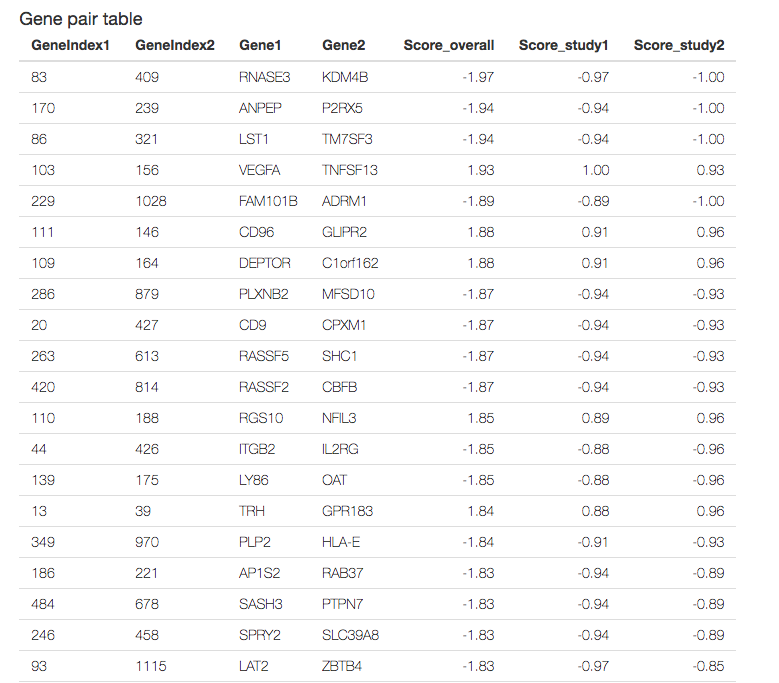
\includegraphics[scale=0.5]{./figure/MetaPredict/MetaPredictresult1.png}
\caption{Results for MetaPredict, top predictive pairs of genes.
A score measures the correlation between the pairs of genes.
}
\label{fig:MetaPredictresult1}
\end{center}
\end{figure}


\begin{figure}[H]
\begin{center}
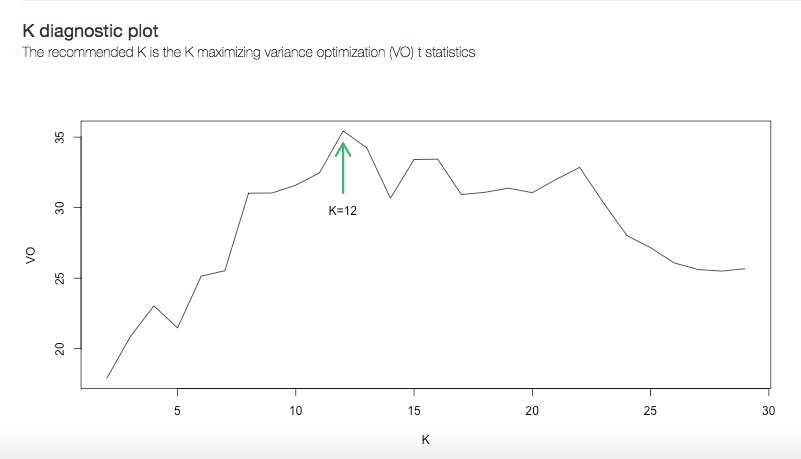
\includegraphics[scale=0.5]{./figure/MetaPredict/MetaPredictresult2.png}
\caption{Results for MetaPredict. 
Select $K$ by maximizing variance optimizaiton (VO) t statistics.
The x-axis is the number of top scoring pairs $K$, 
and the y-axis is the variance optimization (VO) t-statistics.
}
\label{fig:MetaPredictresult2}
\end{center}
\end{figure}


\begin{figure}[H]
\begin{center}
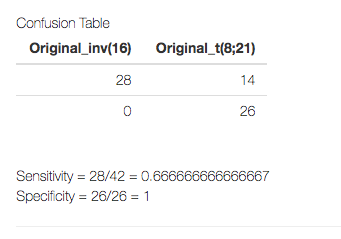
\includegraphics[scale=0.5]{./figure/MetaPredict/MetaPredictresult3.png}
\caption{Confusion table for MetaPredict testing cohort}
\label{fig:MetaPredictresult3}
\end{center}
\end{figure}

\subsubsection{Results}

We used the leukemia data to demonstrate the MetaNetwork module.
After merging the three datasets by filtering 50\% of genes by mean and 50\% by variance, 1283 genes remained.
In this example we only compare two phenotypes: inv(16) and t(15;17). 
Detailed descriptions of these studies can be found in Table~\ref{tab:realDataLeukemia}. 
The top predictive pairs of genes are available in Figure~\ref{fig:MetaPredictresult1}.
The diagnostic plot showing the optimum $K$ is shown in Figure~\ref{fig:MetaPredictresult2}.
A confusion matrix is output,  
showing the prediction results  in Figure \ref{fig:MetaPredictresult3}).
The prediction results are also saved in the working directory.

